% In the batch queue,  queue time becomes dominant but, at the same time, we
% have more freedom to decide the parameters of the slot.

\subsection{Experiments}

In this section we present experiments % that aim
to determine the performances of the NGE and to show how it provides a minimal
overhead while introducing new functionalities.

Experiments % consist in running
run instances of AthenaMP by using NGE pilots, % where each AthenaMP simulates
simulating a pre-determined number of events in the ATLAS detector.\mtnote{are
they 100 events?}\aanote{`Not always.'}
% taken from ATLAS workload.
We present three groups of experiments in which we test the NGE for weak
scalability, weak scalability with multiple generation, and strong scalability.

We % collected data about
measured the execution time of the pilots and of the AthenaMP % that have been
executed within them, collecting timestamps at % by considering
all stages of the execution. Experiments have been performed % out of production
by % using
submitting NGE's pilots % on
to TITAN's batch queue. Because of TITAN's % batch queue
policies, the turnaround time of each run of our experiments is dominated by
% the time spent on TITAN's queue
queue time. Since we are interested only in the performances of the NGE, we
removed queue time from our statistics.

All the experiments have been performed by % setting
configuring AthenaMP
% in such a way that it uses
to use all the 16 cores % present on
of TITAN's worker nodes.


\subsubsection{Weak scalability}

% The
In this experiment % consists in running
we run as many AthenaMP instances (also referred as tasks from now-on) as the number of nodes controlled by the pilot. Each AthenaMP
% have been assigned with 100 events whose simulation requires
simulates 100 events, requiring $\sim 70$ minutes on average.

Tasks do not % experience
wait within the NGE Agent's queue % within the pilot
since % there is
one node %for
is available to each AthenaMP instance. % Therefore, d
Delays in tasks execution are consequence of % only
three other factors: (i) the bootstrapping of the pilot on the nodes; (ii) the
UnitManager, as defined in Section~\ref{sec:arch}, that has to dispatch tasks to
the agent; and (iii) the time that the agent requires to spawn all the tasks on
the nodes.

We tested % different
pilots % sizes, i.e. :
with 250, 500, 1000 and 2000 worker nodes and
%. For all of them, the walltime was
2 hours walltime. Figure~\ref{fig:weakScal1a} depicts the average pilot
duration, the average execution time of AthenaMP, and the pilot's overhead as
function of the pilot size.

\begin{figure}[!htb]
        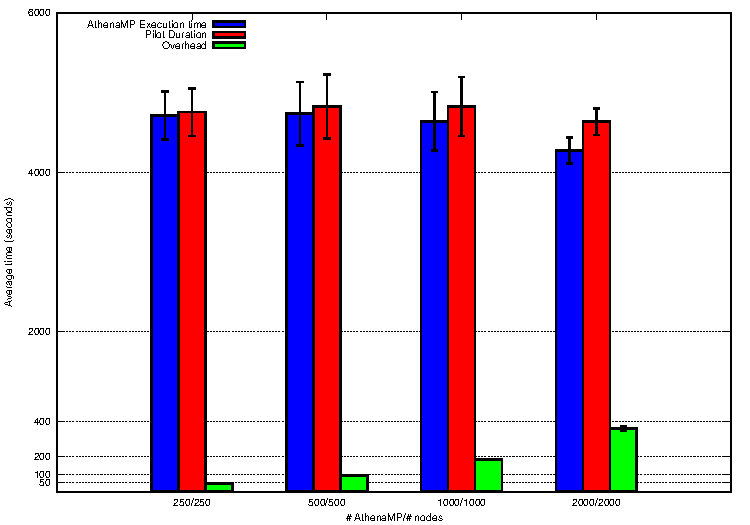
\includegraphics[height=4.5cm,width=\columnwidth]{./figures/NGE/weak1.pdf}
    \caption{Weak scalability: average pilot duration, average duration of a
    single AthenaMP execution, and pilot's overhead for different pilot sizes
    (250, 500, 1000 and 2000 worker nodes). }
\label{fig:weakScal1a}
\end{figure}

% Firstly, w
We % can
observe that, despite some fluctuations due to external factors
% \footnote{such as the
(e.g., Titan's shared filesystem and the shared database used by the NGE), the
average execution time of AthenaMP % oscillates
ranges between 4200 and 4800 seconds. % Secondly, w
We % can
also observe that in all the cases the gap between AthenaMP execution times and
the pilot durations is minimal, although it slightly increases with the pilot
size. % By observing NGE's overhead, w
We % can
notice that NGE's overhead does not grow linearly with the number of units.

%\begin{figure}[!htb]
%        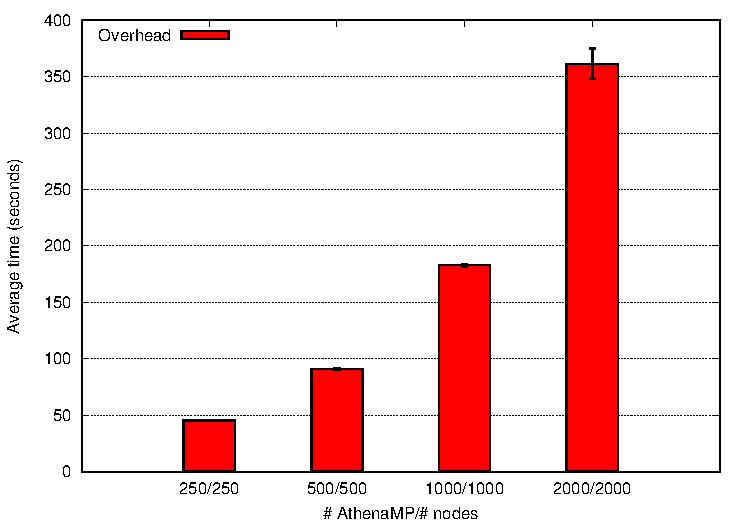
\includegraphics[width=0.4\textwidth]{./figures/NGE/weakOver1.pdf}
%    \caption{Weak scalability: average overhead by running AthenaMP on 200, 500, 1000 and 2000 nodes.}
%\label{fig:weakScal1b}
%\end{figure}


\subsubsection{Weak scalability with multiple generation }

This experiment is similar to the one presented above but, in this case, we want
to test also the impact of submitting multiple generations of % new
AthenaMP to the same pilot.\mtnote{we used `generations' at the beginning of 6,
I am assuming the reader understands the term by now. Please change if you
disagree.}\aanote{I agree}
% instances in place of those that end.
% The reason behind this experiment is to
In this way, we stress the pilot's components, % by pushing new tasks while others are ending their execution
as new tasks are scheduled for execution on the Agent while other tasks are still running.

\mtnote{we do
we need to keep it below 2 hours?}\aanote{You are right. It was misleadind. I Changed. Check if you like it.}
% decided to send for execution a number of AthenaMP instances equal to
We performed the experiment by running five AthenaMP instances per node. % and w
Since we are focusing on the overhead generated by the scheduling and bootstrap of AthenaMP instances, we also reduced  the number of events simulated by each AthenaMP to sixteen in such a way that the running time of each AthenaMP is, on average, $\sim 20$ minutes.
This choice has been made to avoid the wasting of Titan's core hours but it does not affect the aim of the experiment.  
% \footnote{Note that the number of events has been chosen in such a way
% that all the cores of a node run one event.}
%In this way, every core of each worker node was used to simulate one event,
%. This allows us to complete
%reducing the running time of each AthenaMP to ~$20$ minutes. % only.

We tested
% different
pilots
% sizes, i.e. :
with 256, 512, 1024 and 2048 worker nodes and
%. For all of them, the walltime was
3\mtnote{2?} hours walltime. Figure~\ref{fig:weakScal2a} depicts the average
pilot duration, the average execution time of five sequential
generations\mtnote{generations?}\aanote{Changed} of AthenaMP, and the corresponding overhead. We
% can
observe that the difference between the two durations is more marked than in the
previous experiments \mtnote{mostly due to the increased overhead?}\aanote{Well, I guess that's plain.}. Despite this, we can notice that the growth of the overhead is consistent with the increment of the number of tasks per node for pilots with 256, 512 and 1024 worker nodes, and much less than linear for the pilot with 2048 worker nodes \aanote{Although that histogram is not trustworty because it is generate with only two runs.} 

\begin{figure}[!htb]
        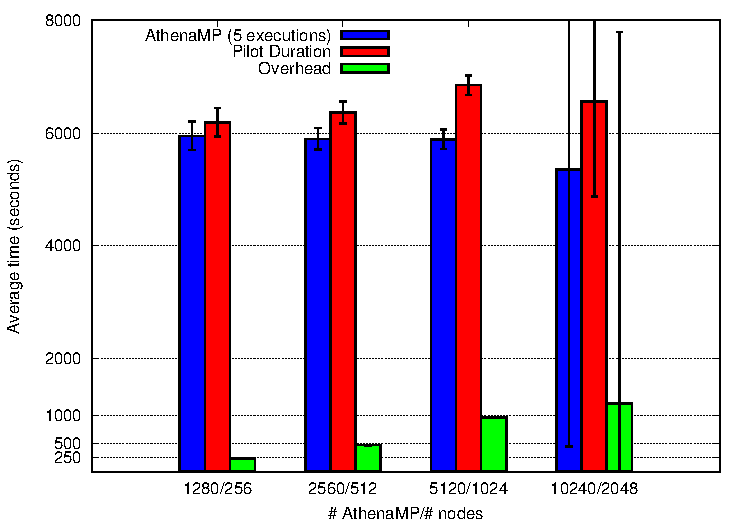
\includegraphics[height=4.5cm,width=\columnwidth]{./figures/NGE/weak2.pdf}
    \caption{Weak scalability with multiple generations: average pilot
    duration, average duration of five sequential AthenaMP executions, and
    pilot's overhead for different pilot sizes (256, 512, 1024 and 2048 nodes).}
\label{fig:weakScal2a}
\end{figure}

%\begin{figure}[!htb]
%        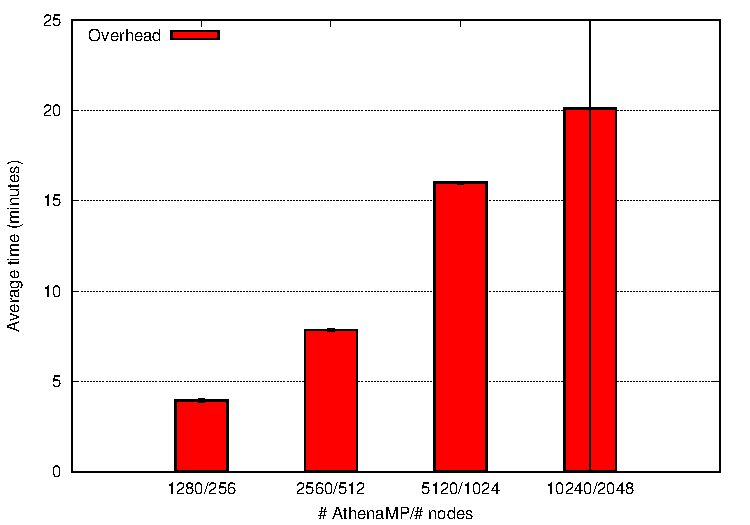
\includegraphics[width=0.4\textwidth]{./figures/NGE/weakOver2.pdf}
%    \caption{Weak scalability with multiple generations: average overhead by running AthenaMP on 256, 512, 1024 and 2048 nodes.}
%\label{fig:weakScal2b}
%\end{figure}


\subsubsection{Strong scalability}

The last experiments % deals with
study strong scalability by running the same amount of tasks for different pilot sizes. We used
% a number of AthenaMP instances equal to
2048 AthenaMP instances and % tested
pilots with 256, 512, 1024 and 2048 nodes. Thus, the number of AthenaMP generations is equal to eight times the size of the smallest pilot and corresponds to the size of the largest pilot. As a consequence, the number of consecutive generations of AthenaMP decreases with the pilot size by generating different dynamics within the pilots. This experiment aim to show that the pilot overhead is not affected by the concurrency level within the pilot but it depends only on the number of tasks.  
\mtnote{Not sure I understand this sentence}\aanote{My fault. It should have been seven and null or 8 and 1. It depends on how we consider the word sequential. anyway, to avoid confusion I changed the sentence.}. Each AthenaMP instance
simulates sixteen events as in the previous experiment.

Figure \ref{fig:strongScala} % depicts
shows the average pilot duration and the average execution time of possibly
sequential AthenaMP instances.  We % can
notice that the difference between the pilot duration and the AthenaMP execution
times is almost constant for all the pilot sizes, although the overall duration
of the pilot decreases linearly with the pilot size.

\begin{figure}[!htb]
        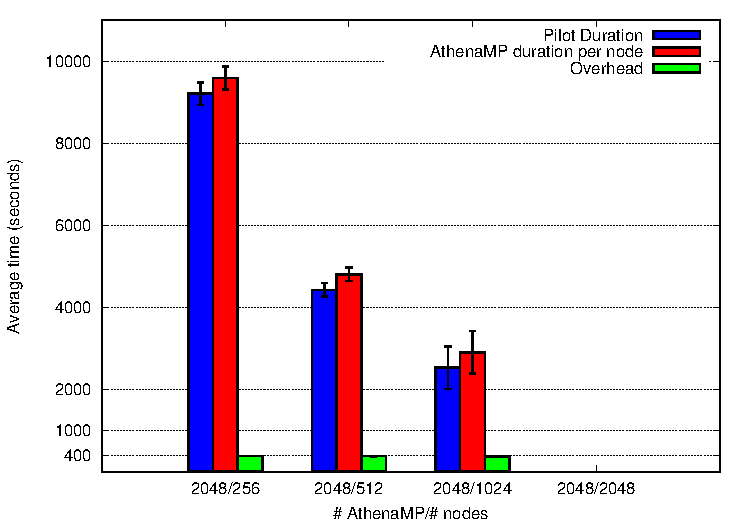
\includegraphics[height=4.5cm,width=\columnwidth]{./figures/NGE/strong.pdf}
    \caption{Strong scalability:  average pilot duration, average duration of
    sequential AthenaMP executions, and pilot's overhead for different pilot
    sizes (256, 512, 1024 and 2048 nodes).}
\label{fig:strongScala}
\end{figure}

%
%\begin{figure}[!htb]
%        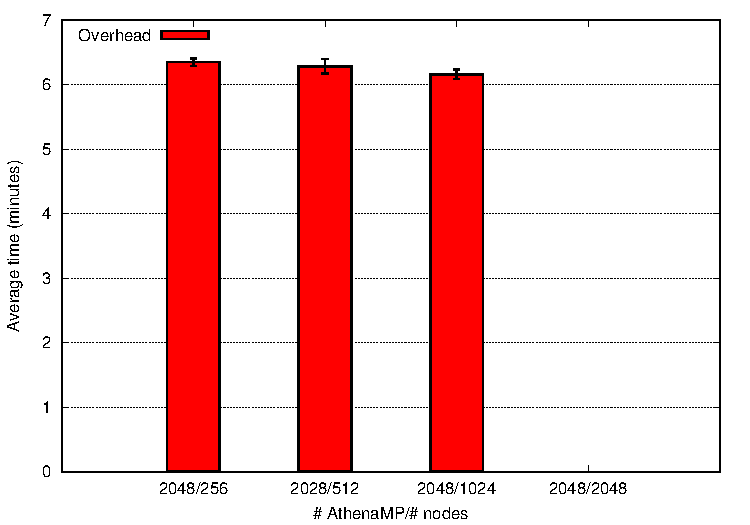
\includegraphics[width=0.4\textwidth]{./figures/NGE/strongOver.pdf}
%    \caption{Strong scalability: average overhead running AthenaMP on 256, 512, 1024 and 2048 nodes.}
%\label{fig:strongScalb}
%\end{figure}

%\subsubsection{Heterogeneous execution}
%
%The last experiment provides a proof of concept about the ability of the NGE to execute heterogeneous workload.
%In particular, we coupled the execution of AthenaMP with the execution of Gromacs to simulate molecular dynamics.
%We performed the experiment by executing at first one AthenaMP per node and then, submitting a Gromacs simulation per core. Each Gromacs simulation requires ~20 minutes.
%We tested the following pilot sizes : 8, 16, 32, 64.
%
%\begin{figure}[!htb]
%        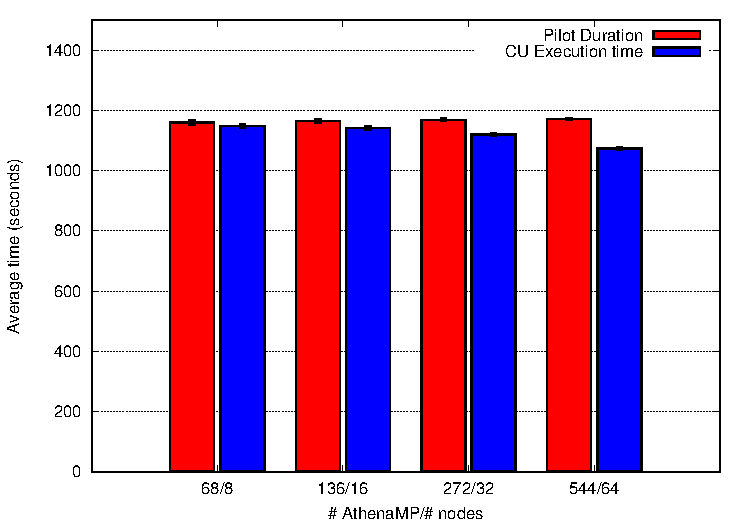
\includegraphics[width=0.5\textwidth]{./figures/NGE/MDET.pdf}
%    \caption{Average pilot execution time against average AthenaMP execution times  for pilot sizes: 256, 512, 1024 and 2048.}
%\label{fig:strongScala}
%\end{figure}
%\begin{figure}[!htb]
%        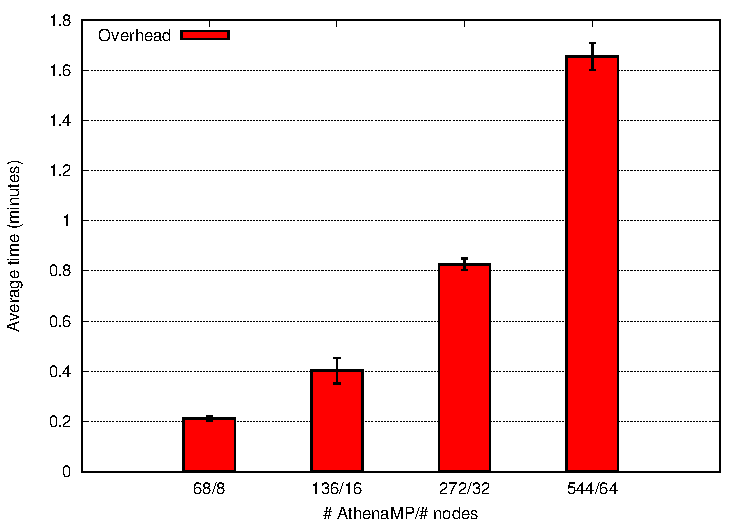
\includegraphics[width=0.5\textwidth]{./figures/NGE/MDOver.pdf}
%    \caption{Average overhead running AthenaMP for pilot sizes: 256, 512, 1024 and 2048.}
%\label{fig:MDScal}
%\end{figure}

% For this reason, the second set of the experiments aims to find
%sub-optimal parameters with which we can minimize the trade-off between the size
%of a slot and the time spent in queue waiting for that slot to become available.
%In other words, we aim to minimize the completion time by finding the best
%trade-off between execution time and queue time.
%
%This execution model introduces slot utilization as one of the key factors for
%high-performances. This happens because, in order to minimize the time spent in
%queue, we might asks for slots in advance and, then we could not be able to
%saturate them when they become available. Thus, this strategy requires a new
%functionality that allows the job to receive and execute new events while it is
%already running on the resources. In order to do that we perform the experiments
%by using a new generation executor that implements such functionality.
%
%As last observation, it is important to point out that the percentage of
%utilization of a slot is minor problem with the current implementation because,
%due to the dynamics of the Backfill queue, PanDA has a high probability to
%re-acquire a slot immediately after it has released one\aanote{Are we able to
%quantify this ``immediately''?}.
